\section{Electromagnetic Waves and Lights}
    \textbf{Refraction} is the bending of light as it propagates from one medium to another. \textbf{Diffraction} is the bending of light as it goes past a barrier. These are wave like properties. 
    \newline \indent
    Newton had a theory, in which indivisible particles of light moved in straight lines and are subject to gravity. Later, Young's famous experiment, essentially the double slit experiment with light, showed that light must be described as a wave since light showed diffraction and interference to form an interference pattern, just like waves. Through this experiment Young was even able to find the wavelengths $\lambda$.
    \newline \indent
    Using Maxwell's equations, for an electric field, the presence of a set of charges oscillating in the $x$-direction allows us to generate a wave equation of the form
    \begin{equation*}
        \frac{\partial^2}{\partial z^2} E_x = \mu_0\epsilon_0\frac{\partial^2}{\partial t^2} E_x
    \end{equation*}
    This equation represents a wave propagating in the $z$-direction with a speed of $v = 1 / \sqrt{\mu_0\epsilon_0}$, which is the speed of light $c$.
    \begin{equation*}
        \frac{1}{\sqrt{\mu_0\epsilon_0}} = c
    \end{equation*} 
    This showed that light was indeed a wave. The same conditions held true for the equation for the magnetic field (in the $y$-direction)
    \begin{equation*}
        \frac{\partial^2}{\partial z^2} B_y = \mu_0\epsilon_0\frac{\partial^2}{\partial t^2} B_y
    \end{equation*}
    There wave equations have general solutions of the form
    \begin{equation*}
        E_x = E_0\cos(kz - \omega t + \varphi) \text{ and  } B_y = B_0\cos(kz - \omega t + \varphi)
    \end{equation*}
    $\varphi$ is the same for each equation because Maxwell's equations require this condition. For this wave, the wavelength $\lambda = 2\pi / k$ and the frequency $f = \omega / 2\pi$ are related by $\lambda f = v - c$.
    \newline \indent $\bullet$
    Nothing restricts the wavelength in the \textbf{electromagnetic spectrum}. Visible light only contains a limited range of wavelengths, but there are infinitely many.
    \newline \indent $\bullet$
    Accelerating charges are necessary to start an electromagnetic wave, but the wave equation does not require any further charges to be present. It does not require a medium, but it can propagate in dielectric media. If the media does not destroy the waves, it is transparent. The only changes are that $\epsilon_0$ must be switched to $\epsilon$ and $\mu_0$ must be switched to $\mu$. So the speed of light in this media is $c' = c/n$ where $n$ is the \textbf{index of refraction}. Transparent materials have $\mu \approx \mu_0$ so $n \approx \sqrt{\kappa}$
    \newline \indent $\bullet$
    Since the electric and magnetic fields have the same phase, when one is at a maximum so is the other; they oscillate together.
    \newline \indent $\bullet$
    In electromagnetic waves $E = vB = cB$ to balance the fields.
    \newline \indent $\bullet$
    The electric and magnetic fields are perpendicular to the direction of wave propagation and to each other. The electromagnetic waves are \textit{transverse}
    \begin{center}
        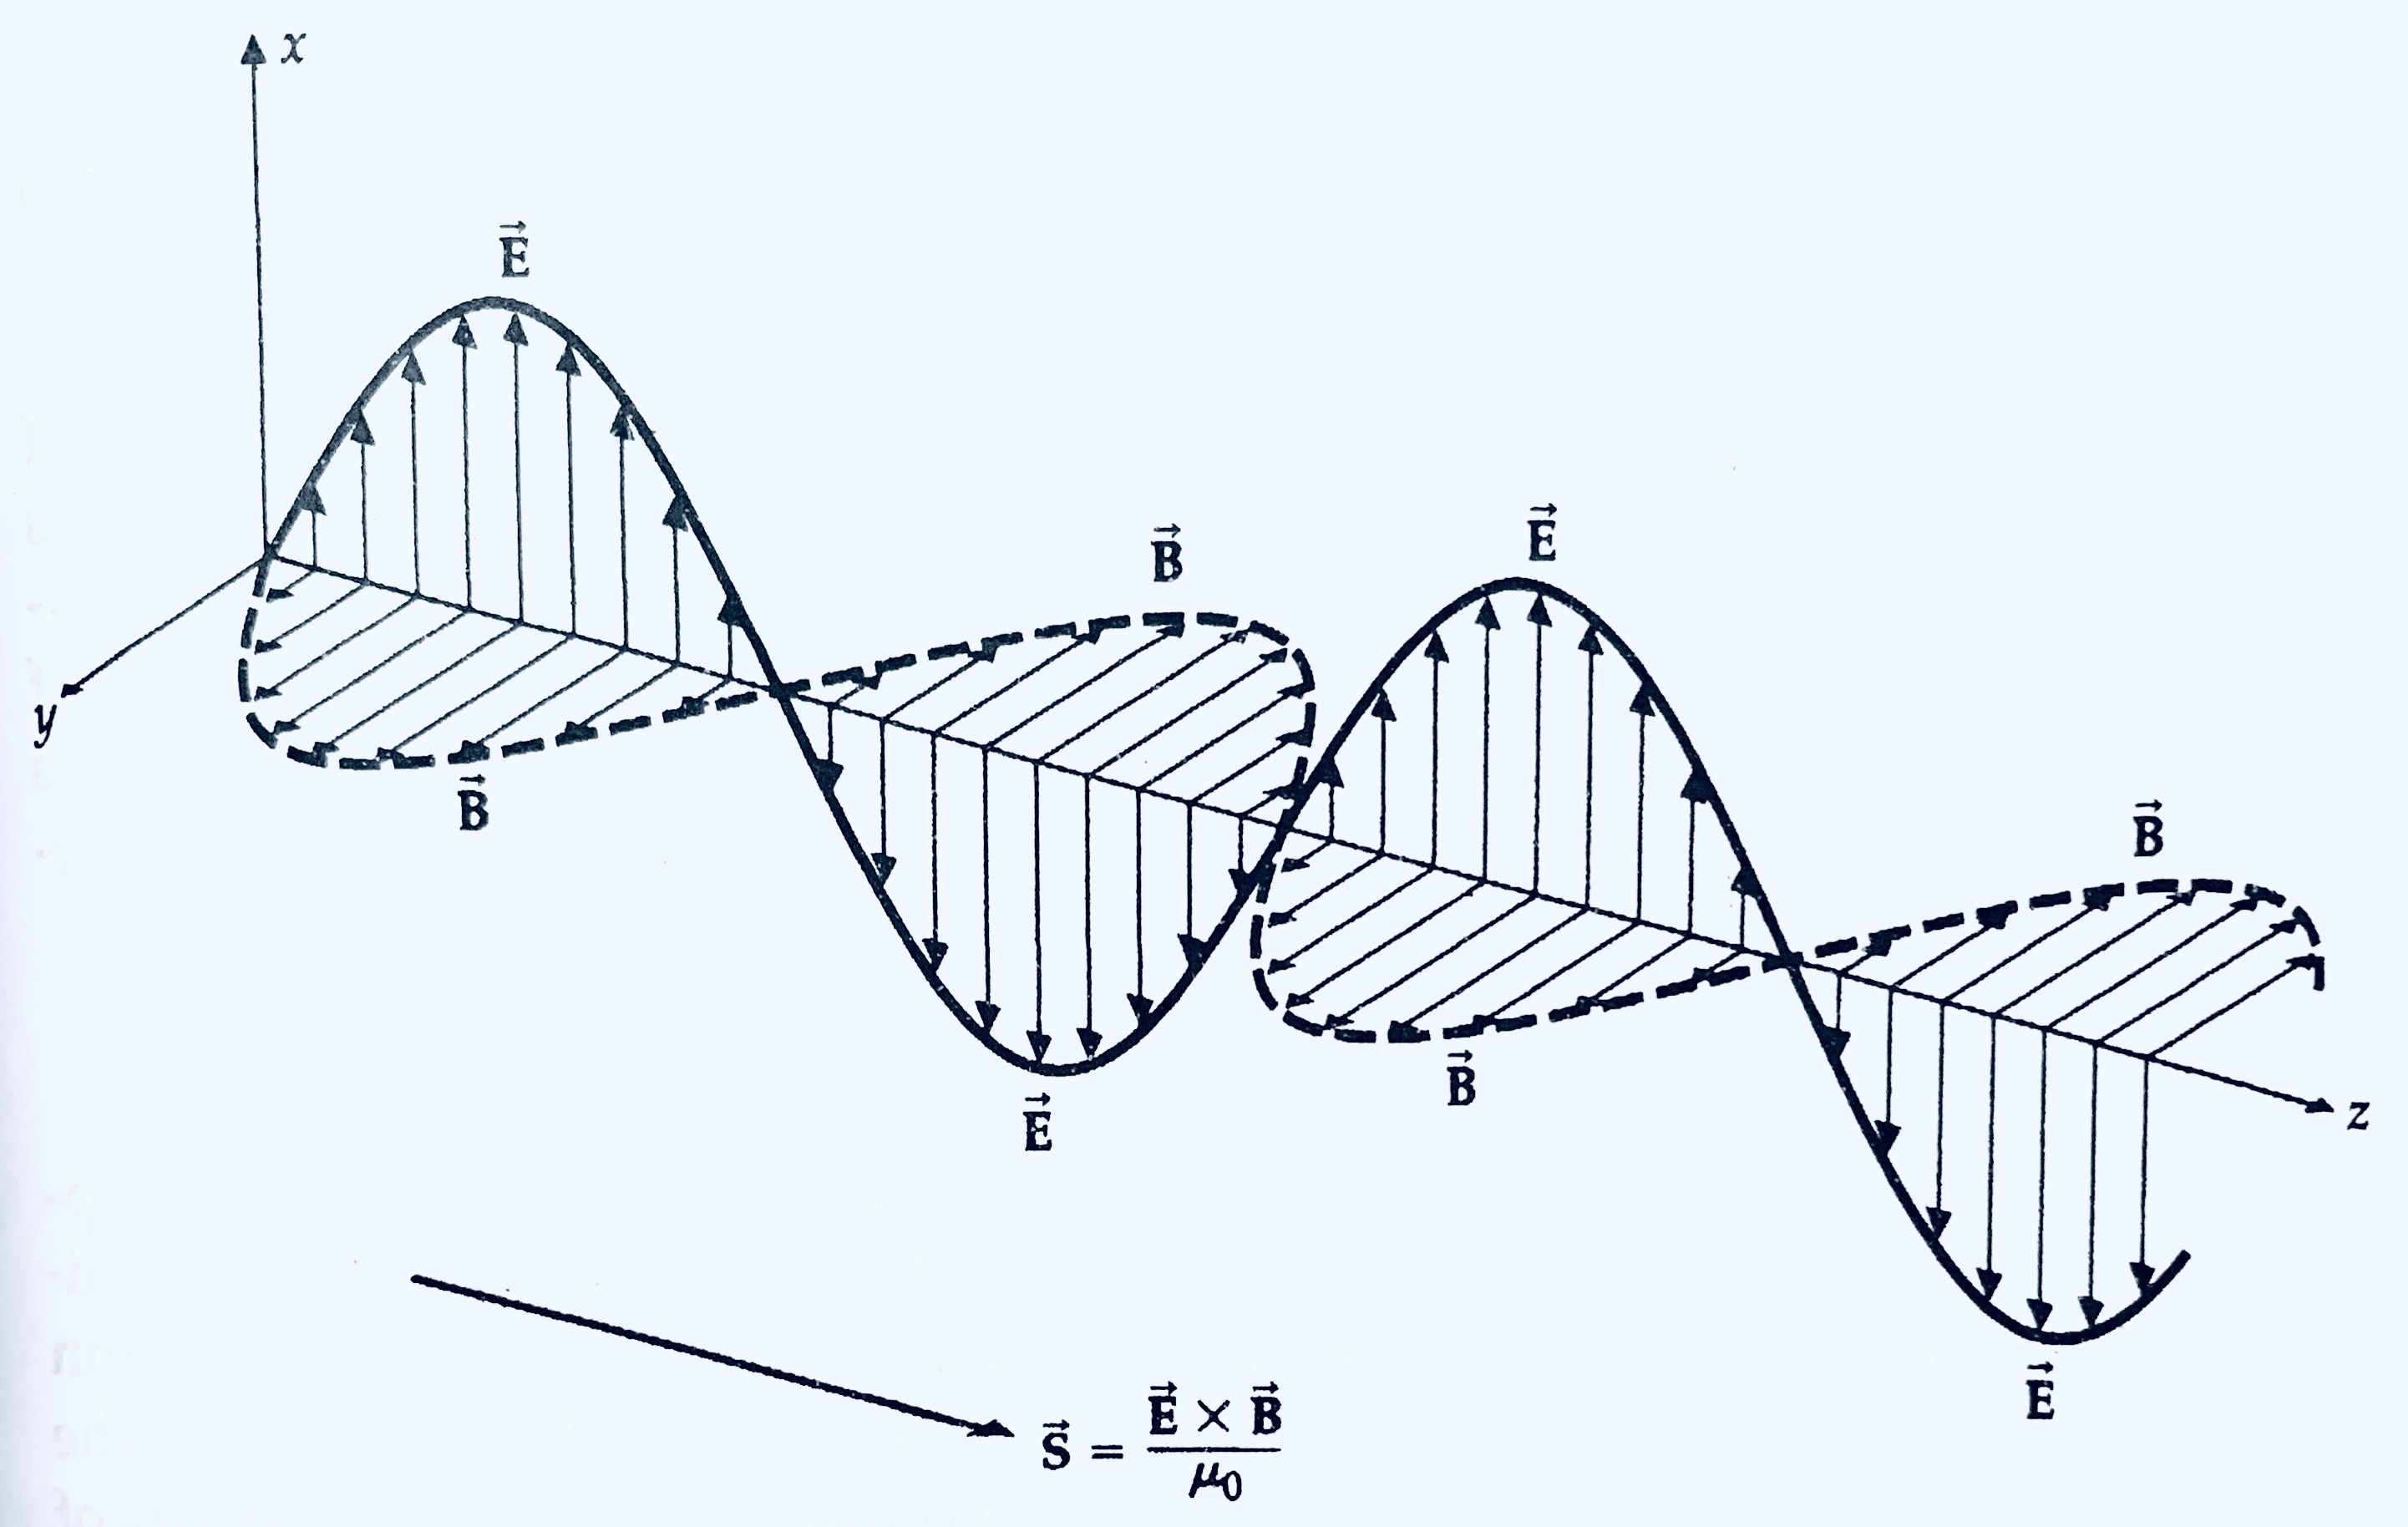
\includegraphics[width=150pt]{electromagnetic.jpg}
    \end{center}
    \begin{center}
        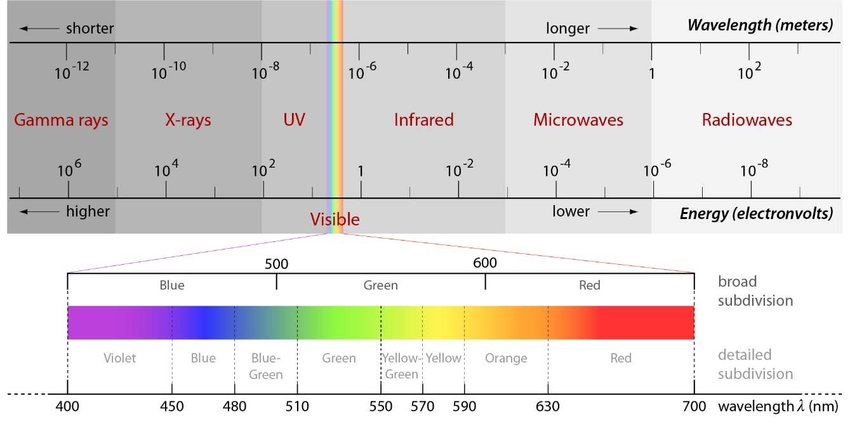
\includegraphics[width=200pt]{spectrum}
    \end{center}
    \subsection*{Energy and Momentum Transport}
    The energy density of electromagnetic waves is
    \begin{equation*}
        u = \frac{1}{2}\epsilon_0(E^2 + c^2B^2) = \epsilon_0 E^2
    \end{equation*}
    since $E = cB$. The energy density is split evenly between the electric and magnet parts of the wave. Also, the energy itself is a wave since it contains $\cos^2(kz - \omega t + \varphi)$ and it propagates with speed $c$. In other words electromagnetic waves transport energy. The rate at which energy arrives at a surface perpendicular to the direction of wave propagation is the \textbf{energy flux} and it is given by $cu$. The energy flux can be more fully characterized by a vector (the \textbf{Poynting vector}) in the direction of $\va{E} \cross \va{B}$ and with magnitude $cu$.
    \begin{equation*}
        \va{S} = (\va{E} \cross \va{B})/\mu_0
    \end{equation*}
    \textbf{Intensity} $I$ is the time average of the energy flux. Since the average of cosine squared is $1/2$, $I = S / 2$.
    \newline \indent
    The electromagnetic fields also exert a net force in the direction of propagation on charged particles, which means the wave also transports momentum to the charge on collision. The momentum per unit volume, or momentum density, is $\va{S}/c^2$. One consequence of this is that the wave exerts pressure on surfaces called \textit{radiation pressure} which is given by $2u$ for a perfectly reflecting surface and $u$ for a perfectly absorbing surface.
    \subsection*{Polarization}
    Although the electric and magnetic fields lies in the plane perpendicular to the direction of propagation, the direction in that plane can be varied. That direction specifies the \textbf{polarization} of the wave. It is possible to measure and filer this direction. A filter that only allows light at a certain angle will reduce the intensity from $I$ to $I\cos^2\theta$ where $\theta$ is the angle between the original polarization and the final polarization. This also reduces the electric field since the filter only uses the component of electric field in the specified direction. The intensity relationship is known as \textit{Malus's law}.